\documentclass{article}
\usepackage{../HW}
\numberwithin{table}{section}
\numberwithin{figure}{section}

\title{COMP3711 Assignment 4}
\begin{document}

\maketitle

\begin{section}{MSTs}
Let $G = (V, E)$ be a weighted undirected connected graph inputted as an adjacency list. Assume that all edges have distinct weights so the \textit{Minimum Spanning Tree} $T$ is unique and that you have already run a MST algorithm that has found and stored T.

Now arbitrarily increase the weight of any one edge $e = (u, v)$ in $E$. You should assume that the edges in the graph still all have distinct weights, i.e, the new weight is different than the weights of all of the other edges.

Let $T'$ be the MST of the graph with the new weights. i.e., after replacing $w(u, v)$ with its new weight $w'(u, v)$.

\begin{enumerate}
    \item Prove that either $T' = T$ or that $T$ and $T'$ differ by at most one edge.
    
    \begin{tcolorbox}[breakable]
    Equivalent to proof: if $e' \neq e$ was an edge in MST before $e$ was changed, then $e'$ will also be in the MST after the weight is changed.
    
    If $e \notin T$, then $T = T'$ as increasing $e$ does not affect the MST. 
    
    If $e = (u, v) \in T$, then we can separate $V$ into $S$ and $V-S$, where $u \in S$ and $v \in V-S$, then $T'$ and $T$ differ by at most only one edge, $e$.  
    
    \textbf{Proof}: 
    \begin{itemize}[noitemsep]
        \item Consider running Prim's Algorithm for $S$ and $V-S$ to build each respective MST separately. By assumption, the weight of each edge is unique, then the MST is unique.
        \item Suppose we run the Prim's algorithm for the subset $S$, and obtained the MST for $S$, namely $T_S$. By repeatedly applying cut lemma, we can expand the MST of $S$, $T_S$ to obtain the MST of $V$, both before and after the weight increase of $e$, $T$ and $T'$. Without loss of generality, we can also find the MST for $V-S$, $T_{S-V}$ is also in $T$ and $T'$. 
        \item In other words, we can split $T$ into three trees, which are $T_S$, $e$, and $T_{V-S}$. and $T'$ into $T_S$, $e^*$, and $T_{V-S}$, where $e^*$ can be the same as $e$ or another edge connecting $S$ and $V-S$. Then, union the MSTs is $MST(S) \cup MST(V-S) = T - e = T' - e^*$.
        \item In either cases, $T_S$ and $T_{V-S}$ is in $T'$
        \item Therefore, at most only one node, $e$ will be changed.
    \end{itemize}
    \end{tcolorbox}

    \item Give an $O(|E|)$ time algorithm for finding $T'$: 
    
    After describing your algorithm, you must then explicitly justify why your algorithm is correct and why it runs in $O(|E|)$ time.
    
    \begin{tcolorbox}
    \begin{enumerate}[(1), noitemsep]
        \item Disconnect the edge $e = (u,v)$ from $T$, where that $v.p = u$. There are two separate trees $u \in T_S$ and $v \in T_{V-S}$, and name the subsets of the nodes in one of the trees as $S$ and $V-S$.
        \item Suppose repeatedly checking the parents of $u$ would return the \textit{root}, $r$, ie. $r.p = r$. Set $v.p \gets v$. Such that repeatedly checking the parents of the items in $S$ would return $r$ and the items in $V-S$ would return $v$. Preprocess the nodes by categorizing the subset of each node by using dynamic programming to check the parent of each node, i.e. the parent of nodes in $S$ is $r$ and the parent of nodes in $V-S$ is $v$. By using stack data structure and dynamic programming, each node will be processed only once, thus the running time is $O(V)$ time.
        \item For each edges $(u,v)$, check if $u \in S$ and $v \in \in V-S$. If so, store the minimum value and the corresponding edge connecting $S$ and $V-S$. Suppose the minimum edge connecting $S$ and $V-S$ is $e'$ after checking all the edges. This procedure checks the edges connecting $S$ and $T-S$ once only, therefore the running time is $O(E)$
        \item Connect back $T_S$ and $T_{V-S}$ with $e'$, return it as $T'$.
    \end{enumerate}
    
    Running time analysis: step (1) takes $O(1)$ amount of time, step (2) takes $O(V)$ amount of time, and step (3) takes $O(E)$ amount of time and step (4) takes $O(1)$ amount of time. Therefore, the total running time is $O(E+V) = O(E)$ because $|E| \geq |V| + 1$.
    \end{tcolorbox}
\end{enumerate}
\end{section}

\newpage
\begin{section}{Graph Algorithms}
Modified from [KT] Chapter 4.

Security analysts are trying to track the spread of an online virus in a
collection of networked computers.

\begin{itemize}
    \item There are $n$ computers in the collection, labelled as $C_1, \dots, C_n$.
    \item The input to the problem is a collection of $m$ \textit{trace-data} triples.
    \item Each triple is of the form $(C_{j_i}, C_{k_i}, t_i) = 1, \dots, m$ where $j_i \neq k_i$. A triple indicates that computer $C_{j_i}$ and computer $C_{k_i}$ exchanged bits at time $t_i$.
    \item You may assume that the triples are sorted in non-decreasing order of time, i.e., $t_i \leq t_{i+1}$ 
\end{itemize}

The analysts would like to be able to answer the following type of question: \textit{If the virus was inserted into computer $C_a$ at time $x$ could it possibly have infected computer $C_b$ by time $y$?}

The mechanics of infection are that: if an infected computer $C_i$ exchanges bits with computer $C_j$ at time $t$ (i.e., either $(C_i, C_j, t)$ or $(C_j, C_i, t)$ appear in the trace data) then $C_j$ becomes immediately infected.

This means that infection spreads from one computer to another through a sequence of communications that occur in non-decreasing order of time. The input to your algorithm also includes the extra information that a specific computer $C_a$ has been infected at time $t_{start}$

Describe an $O(m + n)$ time algorithm which determines, for every other computer, the earliest time at which it can become infected.

More specifically, your algorithm should determine the set $C$ of computers that can be infected by a sequence of communications starting at $C_a$ on or after time $t_{start}$ and then create a directed infection tree $T$ for $C$.

\begin{itemize}
    \item The nodes of $T$ are the computers in $C$. The root of $T$ is $C_a$.
    \item $T$ is represented by two arrays $P[1 \dots n]$ and $Time[1 \dots n]$.
    \item $Time[i]$ should be the earliest time that computer $C_i$ can be infected
    \item Each edge $C_i \rightarrow C_j$ in the tree corresponds to one existing trace-data triple $(C_i, C_j, t)$ or $(C_j, C_i, t)$. \\
    $P [j] = i$ and $Time[j] = t$.
    \item Note that $P [a]$ is undefined and $Time[a] = t_{start}$. \\
    If $C_i \notin C$ then $P [i] = Time[i] = \infty$.
    \item A consequence of the definitions is that $Time[i] \geq Time[P[i]]$ for all $i \neq a$. 
\end{itemize}

\begin{enumerate}
    \item \begin{enumerate}
        \item Give documented pseudocode for creating T and the associated arrays.
        \begin{tcolorbox}[breakable]
        
        \begin{algorithm}[H]
        \LinesNumbered
        \SetKwFunction{Infect}{Infect}
        \SetKwFunction{DFSVisit}{DFS-Visit}
        \SetKwFunction{DFS}{DFS}
        \caption{Infect($n$, $trace$, $C_a$, $t_{start}$)}
        \tcp{Initialize the arrays}
        \KwLet $V[1 \dots n]$ as an array containing $[1 \dots n]$ \\
        \KwLet $u.color \gets white$ for all $u$ in $V$ \tcp*{white for uninfected}
        \KwLet $P[1 \dots n]$ as an array of all $\infty$ \\
        \KwLet $Time[1 \dots n]$ as an array of all $\infty$ \\
        
        \tcp{set the first infection}
        $C_a.color \gets red$ \\
        $P[C_a] = nil$, 
        $Time[C_a] = t_{start}$ \\
        $E = []$, 
        $t = t_{start}$ \\
        \ForEach{$m$ \KwIn $trace$}{
            \tcp{suppose $m[0,1]$ is the edge and $m[2]$ is the time, skip until the t\_start}
            \If{$m[2] < t_{start}$}{
                \KwContinue
            }
            
            \tcp{end of a sequence of trace having the same time}
            \If{$m[2] \neq t$}{
                \tcp{run DFS}
                \DFS{E} \\
                \tcp{reset E and t}
                $t = m[2]$ \\
                $E = []$
            }
            append $(m[0], m[1])$ to $E$
        }
        \tcp{run DFS one last time}
        \DFS{E}\\
        \KwRet P[1 \dots n], Time[1 \dots n]
        \end{algorithm}

        \begin{algorithm}[H]
        \label{alg:p2_DFS}
        \SetKwFunction{DFSVisit}{DFS-Visit}
        \SetKwFunction{DFS}{DFS}
        \SetKwFunction{Build}{Build}
        \caption{DFS(E)}
        \Build{E} \tcp*{initialize adj[1..n] as empty linked lists with size of $n$ and $u.visited \gets false$ for all $u \in V$ with running time of $O(E)$}
        % \KwLet $adj[1 \dots n]$ as array of empty linked lists with size of $n$ \\
        % \KwLet $u.visited \gets false$ for all $u$ in V \\
        \ForEach{$(u, v)$ \KwIn E}{
            append $v$ to $adj[u]$ \\
            append $u$ to $adj[v]$ \\
        }
        \tcp{call DFS if to spread infection, if a node has not been visited previously}
        \ForEach{$(u, v)$ \KwIn E}{
            \If{$u.color = red$ \KwAnd $u.visited = false$}{
                \DFSVisit{u}
            }
            \If{$v.color = red$ \KwAnd $v.visited = false$}{
                \DFSVisit{v}
            }
        }
        \end{algorithm}
        
        \begin{algorithm}[H]
        \SetKwFunction{DFSVisit}{DFS-Visit}
        \tcp{Spread the virus infection to node u}
        \caption{DFS-Visit(u)}
        $u.visited \gets true$ \\
        $u.color \gets red$ \\
        \For{$v$ \KwIn $adj[u]$}{
            \If{$v.color = white$}{
                $P[v] \gets u$ \\
                $Time[v] \gets t$ \\
                $\DFSVisit{v}$
            }
        }
        \end{algorithm}
        \end{tcolorbox}
        
        \item Explain what your code does.
        \begin{tcolorbox}
        The code starts by initializing the $V[1..n]$ by it's label, $P[1 .. n]$ by all $nil$, and $Time[1\dots n]$ by all $\infty$. It also label if a computer has been infected or not by using a $color$ label, where $red$ represent if a computer is already infected and $white$ represent if a computer is not infected yet.
        
        Then, it initialize the virus infection by setting the color of $C_a$, the origin of the virus, as $red$, and setting the initial infection time of $Time[C_a]$, as $t_{start}$.
        
        Define $E$ as an linked list of all edges with the same bit exchange time, and $t$ as the last $trace$ time processed in the following for loop.
        
        Begin the for loop. As the $trace$ is sorted by the bit-exchange time non-descending, we can skip the first few traces before the first infection time $t_{start}$. 
        Then, there would be two cases:
        \begin{itemize}
            \item If the trace time is the same as the previous one, we simply append the edges to $E$
            \item If the trace time is different than the previous one, we run DFS algorithm to see how the virus infection spreads within the tree with the edges $E$ by running the DFS algorithm to update the infection, and fill the $P$ and $Time$ arrays. Then we reset the $t$ to be last trace time, and clear the $E$.
        \end{itemize}
        Then we run the DFS for one last time, as $E$ might not be empty. 
        Finally, return the $P$ and $Time$ arrays.
        \end{tcolorbox}
        
    \end{enumerate}
    \item Prove that your algorithm is correct.

    Please remember to be clear.
    
    Put every new idea and short argument in a separate paragraph with sufficient space between the paragraphs. We can’t understand what you’ve written if we can’t read it.
    
    \begin{tcolorbox}
    The algorithm will check all traces starting from the least time. If some traces shares the same time, the edges will be checked together using the DFS algorithm. The DFS will visit the adjacent nodes if the node is already infected and have not been visited previously in the current DFS call (line 8 and 11 Algorithm \ref{alg:p2_DFS}).
    
    The parent of each node $P[1..n]$ is correct, but not unique. \textbf{Proof:} Note that the $trace$ is sorted by the bit-exchange time in non-decreasing order. For the group of $trace$ with the same time, the algorithm use DFS to track how the infection spreads and set the parent of a node as the other node in the edge where the infection spreads from. In case there are multiple infected nodes connected to a single uninfected node, then the parent of the uninfected node would be chosen by the order of the traces, but choosing the parent of the uninfected node to be other infected node is also correct. Thus, the parent is not unique. Therefore, the algorithm return a correct $P[1..n]$ parent array by considering the correctness of DFS algorithm.
    
    The earliest infection time of each node $Time[1..n]$  is correct and unique. \textbf{Proof:} Note that the $trace$ is sorted by the bit-exchange time in non-decreasing order. For the group of $trace$ with the same time, the algorithm use DFS to track how the infection spreads and set the parent of a node as the other node in the edge where the infection spreads from. Therefore, the algorithm return a correct $Time[1..n]$ parent array. The $Time[1..n]$ array is unique as there must be only one earliest infection time for each node. Therefore the $Time[1..n]$ is correct as each edges is processed order of by the non-decreasing time of the traces, i.e. by uniqueness of earliest infection time, node that is infected earlier must be processed before the node that is infected later, and nodes with the same time will be processed within the same DFS tree.
    
    Therefore, the algorithm return the correct parent array $P[1..n]$ and earliest infection time array $Time[1..n]$
    \end{tcolorbox}
    
    \item Explain why your algorithm runs in $O(m + n)$ time.
    \begin{tcolorbox}
    The initialization of Infect() procedure takes $O(n)$.
    
    The most outer for loop in line 10 of Infect algorithm  runs for all $m$, and call the DFS algorithm. The DFS algorithm will check for all $E$ and run DFS Visit at most once for all nodes in $E$ (Build(E) procedure takes O(E) time). The DFS Visit will visit a node if only the node is never visited previously in the current DFS call. In other word, the running time of DFS(V, E) is $O(|E|)$, as the 'visiting' (line 5-7 of DFS-Visit(u) algorithm) will happen at most once for each node. Suppose $E_i$ is the list of edges in the $i$-th call of DFS algorithm, then $\sum|E_i| \leq m$, as the $|E_i|$ will be cleared everytime DFS is run. 
    
    Therefore the total running time is $O(n + \sum|E_i|) = O(n+m)$ 
    \end{tcolorbox}
\end{enumerate}
\end{section}

\newpage
\begin{section}{BFS and DFS}
In this problem you will have to describe the breadth and depth first search
trees calculated for particular graphs.

\begin{enumerate}[(A)]
    \item Consider the following graph $G = (V, E)$ with 16 vertices
    
    $V = \cbracket{u_0, \dots, u_7} \cup \cbracket{v_0, \dots, v_7}$ and the edges $E$ as given by the following adjacency lists:
    
    Each node ${u_i}$ in $\cbracket{u_0, \dots, u_7}$ is connected, in the following order, to its four neighbors: $u_{(i+1) \mod 8}$, $u_{(i-1) \mod 8}$, $v_{(i+1) \mod 8}$, $v_{(i-1) \mod 8}$.
    
    Each node ${v_i}$ in $\cbracket{v_0, \dots, v_7}$ is connected, in the following order, to its four neighbors: $u_{(i+1) \mod 8}$, $u_{(i-1) \mod 8}$, $v_{(i+3) \mod 8}$, $v_{(i-3) \mod 8}$.
\begin{figure}[h!]
    \centering
    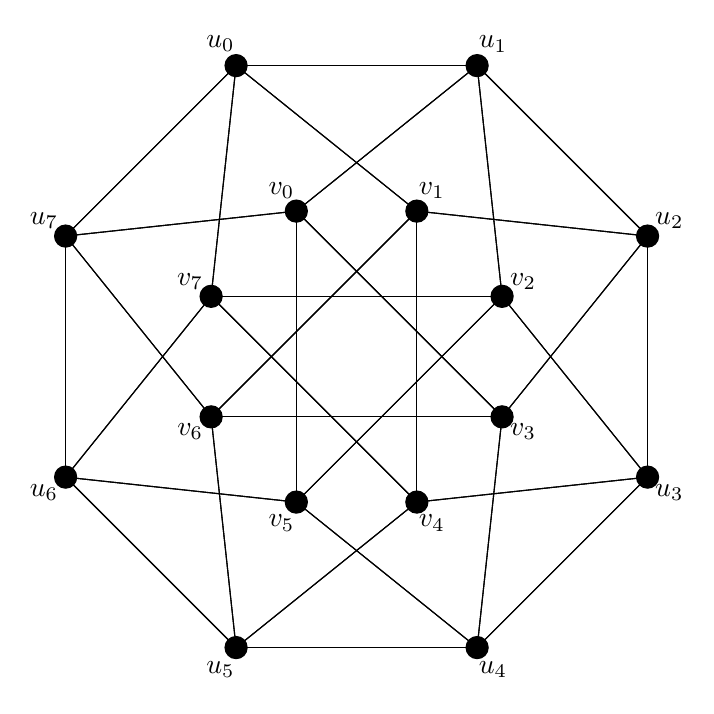
\begin{tikzpicture}[bullet/.style={circle,fill,minimum size=8pt,
              inner sep=0pt, outer sep=0pt},nodes=bullet]
        \foreach \i[
            evaluate = \i as \ti using {112.5 - (\i)*45}
            ] in {0,...,7}{
            \node[draw, label={\ti:$v_\i$}] (v\i) at (\ti : 2cm) {};
            \node[draw, label={\ti:$u_\i$}] (u\i) at (\ti : 4cm) {};
        };
        \foreach \i [
            evaluate = \i as \A using {int(mod(\i + 1, 8))},
            evaluate = \i as \B using {int(mod(8 + \i - 1, 8))},
            evaluate = \i as \C using {int(mod(\i + 1, 8))},
            evaluate = \i as \D using {int(mod(8 + \i - 1, 8))},
        ] in {0,...,7}{
            \draw (u\i) -- (u\A);
            \draw (u\i) -- (u\B);
            \draw (u\i) -- (v\C);
            \draw (u\i) -- (v\D);
        };
        \foreach \i [
            evaluate = \i as \A using {int(mod(\i + 1, 8))},
            evaluate = \i as \B using {int(mod(8 + \i - 1, 8))},
            evaluate = \i as \C using {int(mod(\i + 3, 8))},
            evaluate = \i as \D using {int(mod(8 + \i - 3, 8))},
        ] in {0,...,7}{
            \draw (v\i) -- (u\A);
            \draw (v\i) -- (u\B);
            \draw (v\i) -- (v\C);
            \draw (v\i) -- (v\D);
        };
    \end{tikzpicture}
    \caption{Graph with all edges}
    \label{fig:p3_1}
\end{figure}
\newpage
\begin{enumerate}
    \item  Recall that BFS is \textit{Breadth First Search}. Draw the edges of the BFS tree of $G$ that results when starting from the node $\mathbf{u_1}$, with $G$ represented using the adjacency lists described above.
    \begin{tcolorbox}[breakable]
        \begin{figure}[H]
            \centering
            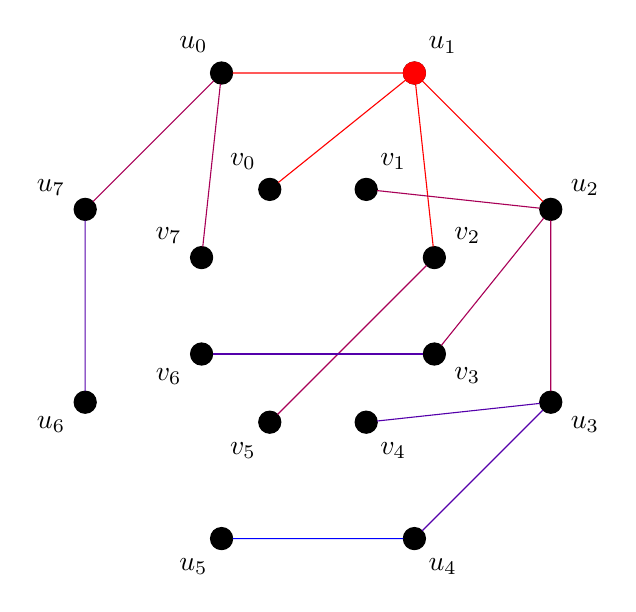
\begin{tikzpicture}[bullet/.style={circle,fill,minimum size=8pt,
              inner sep=0pt, outer sep=0pt}, scale=0.8]
                \foreach \i[
                    evaluate = \i as \ti using {112.5 - (\i)*45}
                    ] in {0,...,7}{
                    \node[draw, bullet, label={\ti:$v_\i$}] (v\i) at (\ti : 2cm) {};
                    \node[draw, bullet, label={\ti:$u_\i$}] (u\i) at (\ti : 4cm) {};
                };
                \node[draw, red, bullet] at (u1) {};
                \draw[draw={red!100!blue}] (u1) -- (u2) {};
                \draw[draw={red!100!blue}] (u1) -- (u0) {};
                \draw[draw={red!100!blue}] (u1) -- (v2) {};
                \draw[draw={red!100!blue}] (u1) -- (v0) {};
                \draw[draw={red!66!blue}] (u2) -- (u3) {};
                \draw[draw={red!66!blue}] (u2) -- (v3) {};
                \draw[draw={red!66!blue}] (u2) -- (v1) {};
                \draw[draw={red!66!blue}] (u0) -- (u7) {};
                \draw[draw={red!66!blue}] (u0) -- (v7) {};
                \draw[draw={red!66!blue}] (v2) -- (v5) {};
                \draw[draw={red!33!blue}] (u3) -- (u4) {};
                \draw[draw={red!33!blue}] (u3) -- (v4) {};
                \draw[draw={red!33!blue}] (v3) -- (v6) {};
                \draw[draw={red!33!blue}] (u7) -- (u6) {};
                \draw[draw={red!0!blue}] (u4) -- (u5) {};
            
            \end{tikzpicture}

            \caption{BFS Tree}
            \label{fig:p3_2}
        \end{figure}
    \end{tcolorbox}
        \item Recall that DFS is \textit{Depth First Search}. Draw the edges of the BFS tree of $G$ that results when starting from the node $\mathbf{u_1}$, with $G$ represented using the adjacency lists described above.
    
    \begin{tcolorbox}
        \begin{figure}[H]
            \centering
            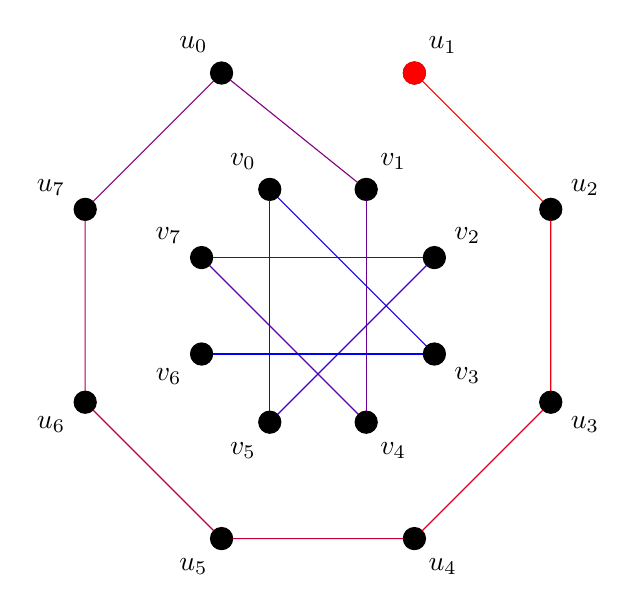
\begin{tikzpicture}[bullet/.style={circle,fill,minimum size=8pt,
              inner sep=0pt, outer sep=0pt}, scale=0.8]
                \foreach \i[
                    evaluate = \i as \ti using {112.5 - (\i)*45}
                    ] in {0,...,7}{
                    \node[draw, bullet, label={\ti:$v_\i$}] (v\i) at (\ti : 2cm) {};
                    \node[draw, bullet, label={\ti:$u_\i$}] (u\i) at (\ti : 4cm) {};
                };
                \node[draw, red, bullet] at (u1) {};
                \draw[draw={red!100!blue}] (u1) -- (u2) {};
                \draw[draw={red!93!blue}] (u2) -- (u3) {};
                \draw[draw={red!86!blue}] (u3) -- (u4) {};
                \draw[draw={red!79!blue}] (u4) -- (u5) {};
                \draw[draw={red!72!blue}] (u5) -- (u6) {};
                \draw[draw={red!65!blue}] (u6) -- (u7) {};
                \draw[draw={red!58!blue}] (u7) -- (u0) {};
                \draw[draw={red!50!blue}] (u0) -- (v1) {};
                \draw[draw={red!43!blue}] (v1) -- (v4) {};
                \draw[draw={red!36!blue}] (v4) -- (v7) {};
                \draw[draw={red!29!blue}] (v7) -- (v2) {};
                \draw[draw={red!22!blue}] (v2) -- (v5) {};
                \draw[draw={red!15!blue}] (v5) -- (v0) {};
                \draw[draw={red!8!blue}] (v0) -- (v3) {};
                \draw[draw={red!0!blue}] (v3) -- (v6) {};
            \end{tikzpicture}
            \caption{DFS Tree}
            \label{fig:p3_2}
        \end{figure}
    \end{tcolorbox}
\end{enumerate}

\newpage
\item Consider the same graph $G = (V, E)$ shown above and the same adjacency lists as illustrated in (A).
\begin{enumerate}
\item  Recall that BFS is \textit{Breadth First Search}. Draw the edges of the BFS tree of $G$ that results when starting from the node $\mathbf{v_1}$, with $G$ represented using the adjacency lists described above.
\begin{tcolorbox}[breakable]
    \begin{figure}[H]
        \centering
        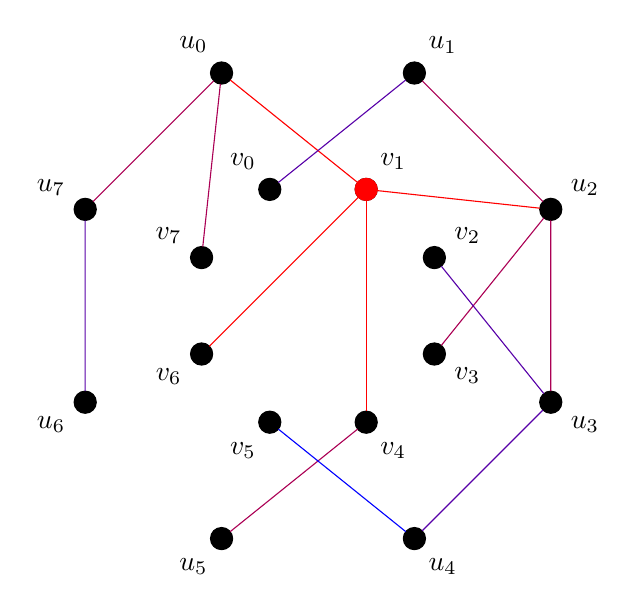
\begin{tikzpicture}[bullet/.style={circle,fill,minimum size=8pt,
          inner sep=0pt, outer sep=0pt}, scale=0.8]
            \foreach \i[
                evaluate = \i as \ti using {112.5 - (\i)*45}
                ] in {0,...,7}{
                \node[draw, bullet, label={\ti:$v_\i$}] (v\i) at (\ti : 2cm) {};
                \node[draw, bullet, label={\ti:$u_\i$}] (u\i) at (\ti : 4cm) {};
            };
            \node[draw, red, bullet] at (v1) {};
            \draw[draw={red!100!blue}] (v1) -- (u2) {};
            \draw[draw={red!100!blue}] (v1) -- (u0) {};
            \draw[draw={red!100!blue}] (v1) -- (v4) {};
            \draw[draw={red!100!blue}] (v1) -- (v6) {};
            \draw[draw={red!67!blue}] (u2) -- (u3) {};
            \draw[draw={red!67!blue}] (u2) -- (u1) {};
            \draw[draw={red!67!blue}] (u2) -- (v3) {};
            \draw[draw={red!67!blue}] (u0) -- (u7) {};
            \draw[draw={red!67!blue}] (u0) -- (v7) {};
            \draw[draw={red!67!blue}] (v4) -- (u5) {};
            \draw[draw={red!34!blue}] (u3) -- (u4) {};
            \draw[draw={red!34!blue}] (u3) -- (v2) {};
            \draw[draw={red!34!blue}] (u1) -- (v0) {};
            \draw[draw={red!34!blue}] (u7) -- (u6) {};
            \draw[draw={red!0!blue}] (u4) -- (v5) {};
        \end{tikzpicture}

        \caption{BFS Tree}
        \label{fig:p3_2}
    \end{figure}
\end{tcolorbox}
\item Recall that DFS is \textit{Depth First Search}. Draw the edges of the BFS tree of $G$ that results when starting from the node $\mathbf{v_1}$, with $G$ represented using the adjacency lists described above.

\begin{tcolorbox}
    \begin{figure}[H]
        \centering
        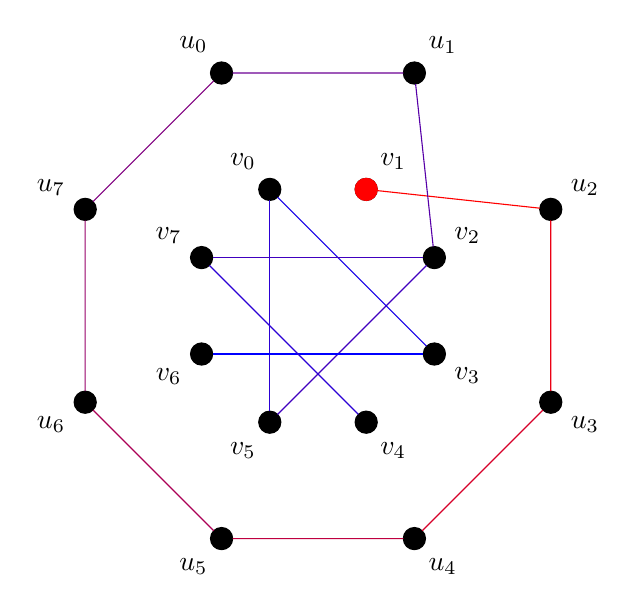
\begin{tikzpicture}[bullet/.style={circle,fill,minimum size=8pt,
          inner sep=0pt, outer sep=0pt}, scale=0.8]
            \foreach \i[
                evaluate = \i as \ti using {112.5 - (\i)*45}
                ] in {0,...,7}{
                \node[draw, bullet, label={\ti:$v_\i$}] (v\i) at (\ti : 2cm) {};
                \node[draw, bullet, label={\ti:$u_\i$}] (u\i) at (\ti : 4cm) {};
            };
            \node[draw, red, bullet] at (v1) {};
            \draw[draw={red!100!blue}] (v1) -- (u2) {};
            \draw[draw={red!92!blue}] (u2) -- (u3) {};
            \draw[draw={red!84!blue}] (u3) -- (u4) {};
            \draw[draw={red!75!blue}] (u4) -- (u5) {};
            \draw[draw={red!67!blue}] (u5) -- (u6) {};
            \draw[draw={red!59!blue}] (u6) -- (u7) {};
            \draw[draw={red!50!blue}] (u7) -- (u0) {};
            \draw[draw={red!42!blue}] (u0) -- (u1) {};
            \draw[draw={red!34!blue}] (u1) -- (v2) {};
            \draw[draw={red!25!blue}] (v2) -- (v5) {};
            \draw[draw={red!17!blue}] (v5) -- (v0) {};
            \draw[draw={red!9!blue}] (v0) -- (v3) {};
            \draw[draw={red!0!blue}] (v3) -- (v6) {};
            \draw[draw={red!25!blue}] (v2) -- (v7) {};
            \draw[draw={red!17!blue}] (v7) -- (v4) {};
        \end{tikzpicture}
        \caption{DFS Tree}
        \label{fig:p3_2}
    \end{figure}
\end{tcolorbox}
\end{enumerate}
\end{enumerate}
\end{section}

\newpage
\begin{section}{Find Minimum Spanning Tree (MST) and Shortest Path}
The tourist map of Venice can be modeled as a connected, edge-weighted undirected graph with nodes being its major attractions and edges being tourist routes connecting two attractions.

\begin{figure}[h]
    \centering
    \resizebox{0.7\linewidth}{!}{
    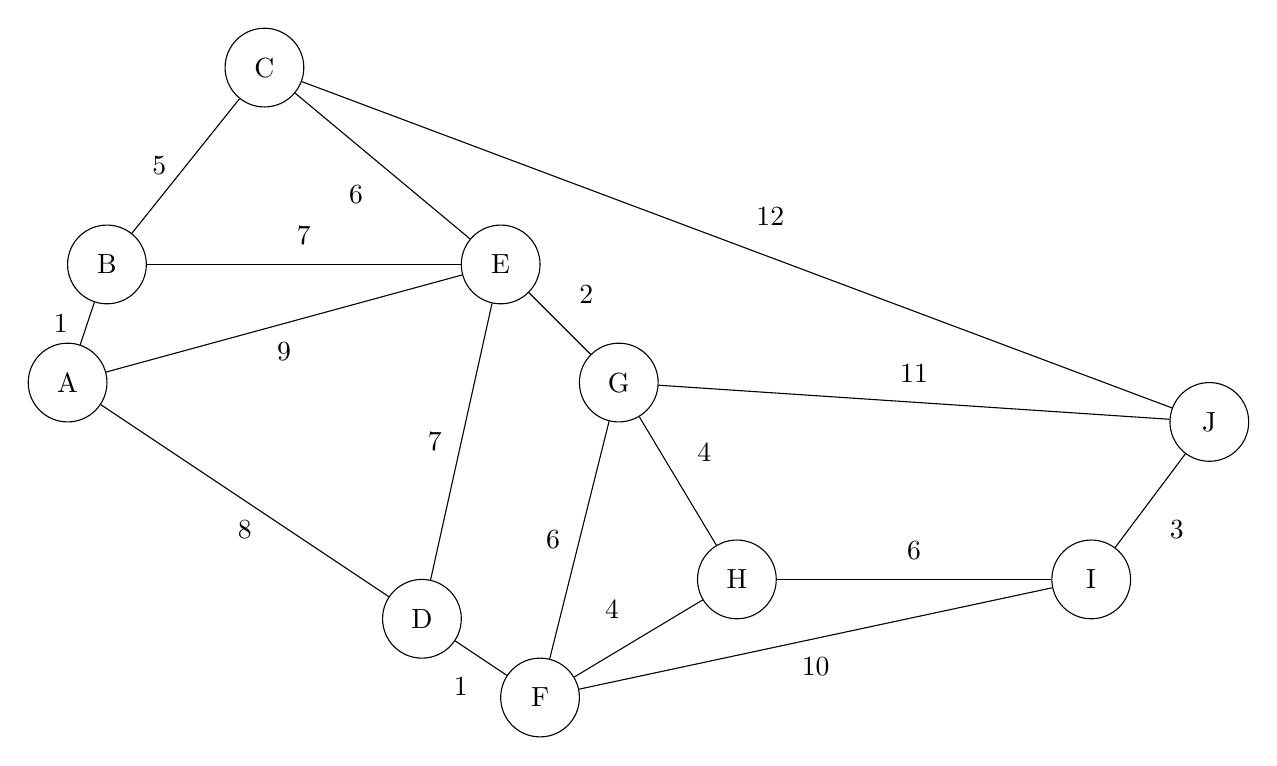
\begin{tikzpicture}[
        roundnode/.style={
            draw, circle, minimum size=1cm
        }
    ]
    \node[roundnode] (A) at (0, 0) {A};
    \node[roundnode] (B) at (0.5, 1.5) {B};
    \node[roundnode] (C) at (2.5, 4) {C};
    \node[roundnode] (D) at (4.5, -3) {D};
    \node[roundnode] (E) at (5.5, 1.5) {E};
    \node[roundnode] (F) at (6, -4) {F};
    \node[roundnode] (G) at (7, 0) {G};
    \node[roundnode] (H) at (8.5, -2.5) {H};
    \node[roundnode] (I) at (13, -2.5) {I};
    \node[roundnode] (J) at (14.5, -0.5) {J};
    
    % nodes
    \draw (A) -- (B) node[midway, label={180:$1$}] {};
    \draw (A) -- (D) node[midway, label={270:$8$}] {};
    \draw (A) -- (E) node[midway, label={270:$9$}] {};
    \draw (B) -- (C) node[midway, label={180:$5$}] {};
    \draw (B) -- (E) node[midway, label={90:$7$}] {};
    \draw (C) -- (E) node[midway, label={225:$6$}] {};
    \draw (C) -- (J) node[midway, label={45:$12$}] {};
    \draw (D) -- (E) node[midway, label={180:$7$}] {};
    \draw (D) -- (F) node[midway, label={250:$1$}] {};
    \draw (E) -- (G) node[midway, label={45:$2$}] {};
    \draw (F) -- (G) node[midway, label={180:$6$}] {};
    \draw (F) -- (H) node[midway, label={135:$4$}] {};
    \draw (F) -- (I) node[midway, label={270:$10$}] {};
    \draw (G) -- (H) node[midway, label={45:$4$}] {};
    \draw (G) -- (J) node[midway, label={90:$11$}] {};
    \draw (H) -- (I) node[midway, label={90:$6$}] {};
    \draw (I) -- (J) node[midway, label={315:$3$}] {};
    \end{tikzpicture}
    }
    \caption{Undirected graph of the map}
    \label{fig:p4_1}
\end{figure}


\begin{enumerate}[(A)]
    \item The following graph depicts the tourist routes and their corresponding distance in terms of kilometers among 10 major Venice attractions shown in the following figures.
    
    \begin{enumerate}[(a)]
        \item Run \textbf{Prim’s} algorithm taught in 16\_MST on the graph, \textit{starting from vertex $A$}, to find $G$’s MST. (This minimizes the total distance covered, in kilometers, of the spanning tree.). provide the following information for each step:
        \begin{enumerate}[(1)]
            \item $S$ that keeps the current explored nodes; initially $S = \cbracket{A}$
            \item $T$ that keeps the current selected MST edges; initially $T = \cbracket{}$
            \item A table that tracks the key value and parent of each node.
            
            Also, upon completion of the algorithm, please:
            \item draw the final MST, and
            \item provide the minimum total route length (in kilometers) achieved by this MST.
        \end{enumerate}
        
        \begin{tcolorbox}[breakable]
        \begin{enumerate}[(1)]
            % \item Step 0:
            % $$S = \cbracket{A}$$
            % $$T = \cbracket{}$$
            % \begin{table}[H]
            %     \centering
            %     \begin{tabular}{c|cccccccccc}
            %         \hline
            %         Node &  A & B & C & D & E & F & G & H & I & J \\
            %         Key & & & & & & & & & & \\
            %         Parent & & & & & & & & & & \\
            %         \hline
            %     \end{tabular}
            % \end{table}

            \item Step 0:
            $$S = \cbracket{A}$$
            $$T = \cbracket{}$$
            \begin{table}[H]
                \centering
                \begin{tabular}{c|cccccccccc}
                    \hline
                    Node & A & B & C & D & E & F & G & H & I & J \\
                    Key & 0 & 1 & $\infty$ & 8 & 9 & $\infty$ & $\infty$ & $\infty$ & $\infty$ & $\infty$ \\
                    Parent & - & A & - & A & A & - & - & - & - & - \\
                    \hline
                \end{tabular}
            \end{table}
        

            \item Step 1:
            $$S = \cbracket{A, B}$$
            $$T = \cbracket{(A, B)}$$
            \begin{table}[H]
                \centering
                \begin{tabular}{c|cccccccccc}
                    \hline
                    Node & A & B & C & D & E & F & G & H & I & J \\
                    Key & 0 & 1 & 5 & 8 & 7 & $\infty$ & $\infty$ & $\infty$ & $\infty$ & $\infty$ \\
                    Parent & - & A & B & A & B & - & - & - & - & - \\
                    \hline
                \end{tabular}
            \end{table}
        

            \item Step 2:
            $$S = \cbracket{A, B, C}$$
            $$T = \cbracket{(A, B), (B, C)}$$
            \begin{table}[H]
                \centering
                \begin{tabular}{c|cccccccccc}
                    \hline
                    Node & A & B & C & D & E & F & G & H & I & J \\
                    Key & 0 & 1 & 5 & 8 & 6 & $\infty$ & $\infty$ & $\infty$ & $\infty$ & 12 \\
                    Parent & - & A & B & A & C & - & - & - & - & C \\
                    \hline
                \end{tabular}
            \end{table}
        

            \item Step 3:
            $$S = \cbracket{A, B, C, E}$$
            $$T = \cbracket{(A, B), (B, C), (C, E)}$$
            \begin{table}[H]
                \centering
                \begin{tabular}{c|cccccccccc}
                    \hline
                    Node & A & B & C & D & E & F & G & H & I & J \\
                    Key & 0 & 1 & 5 & 7 & 6 & $\infty$ & 2 & $\infty$ & $\infty$ & 12 \\
                    Parent & - & A & B & E & C & - & E & - & - & C \\
                    \hline
                \end{tabular}
            \end{table}
        

            \item Step 4:
            $$S = \cbracket{A, B, C, E, G}$$
            $$T = \cbracket{(A, B), (B, C), (C, E), (E, G)}$$
            \begin{table}[H]
                \centering
                \begin{tabular}{c|cccccccccc}
                    \hline
                    Node & A & B & C & D & E & F & G & H & I & J \\
                    Key & 0 & 1 & 5 & 7 & 6 & 6 & 2 & 4 & $\infty$ & 11 \\
                    Parent & - & A & B & E & C & G & E & G & - & G \\
                    \hline
                \end{tabular}
            \end{table}
        

            \item Step 5:
            $$S = \cbracket{A, B, C, E, G, H}$$
            $$T = \cbracket{(A, B), (B, C), (C, E), (E, G), (G, H)}$$
            \begin{table}[H]
                \centering
                \begin{tabular}{c|cccccccccc}
                    \hline
                    Node & A & B & C & D & E & F & G & H & I & J \\
                    Key & 0 & 1 & 5 & 7 & 6 & 4 & 2 & 4 & 6 & 11 \\
                    Parent & - & A & B & E & C & H & E & G & H & G \\
                    \hline
                \end{tabular}
            \end{table}
        

            \item Step 6:
            $$S = \cbracket{A, B, C, E, G, H, F}$$
            $$T = \cbracket{(A, B), (B, C), (C, E), (E, G), (G, H), (H, F)}$$
            \begin{table}[H]
                \centering
                \begin{tabular}{c|cccccccccc}
                    \hline
                    Node & A & B & C & D & E & F & G & H & I & J \\
                    Key & 0 & 1 & 5 & 1 & 6 & 4 & 2 & 4 & 6 & 11 \\
                    Parent & - & A & B & F & C & H & E & G & H & G \\
                    \hline
                \end{tabular}
            \end{table}
        

            \item Step 7:
            $$S = \cbracket{A, B, C, E, G, H, F, D}$$
            $$T = \cbracket{(A, B), (B, C), (C, E), (E, G), (G, H), (H, F), (F, D)}$$
            \begin{table}[H]
                \centering
                \begin{tabular}{c|cccccccccc}
                    \hline
                    Node & A & B & C & D & E & F & G & H & I & J \\
                    Key & 0 & 1 & 5 & 1 & 6 & 4 & 2 & 4 & 6 & 11 \\
                    Parent & - & A & B & F & C & H & E & G & H & G \\
                    \hline
                \end{tabular}
            \end{table}
        

            \item Step 8:
            $$S = \cbracket{A, B, C, E, G, H, F, D, I}$$
            $$T = \cbracket{(A, B), (B, C), (C, E), (E, G), (G, H), (H, F), (F, D), (H, I)}$$
            \begin{table}[H]
                \centering
                \begin{tabular}{c|cccccccccc}
                    \hline
                    Node & A & B & C & D & E & F & G & H & I & J \\
                    Key & 0 & 1 & 5 & 1 & 6 & 4 & 2 & 4 & 6 & 3 \\
                    Parent & - & A & B & F & C & H & E & G & H & I \\
                    \hline
                \end{tabular}
            \end{table}
        

            \item Step 9:
            $$S = \cbracket{A, B, C, E, G, H, F, D, I, J}$$
            $$T = \cbracket{(A, B), (B, C), (C, E), (E, G), (G, H), (H, F), (F, D), (H, I), (I, J)}$$
            \begin{table}[H]
                \centering
                \begin{tabular}{c|cccccccccc}
                    \hline
                    Node & A & B & C & D & E & F & G & H & I & J \\
                    Key & 0 & 1 & 5 & 1 & 6 & 4 & 2 & 4 & 6 & 3 \\
                    Parent & - & A & B & F & C & H & E & G & H & I \\
                    \hline
                \end{tabular}
            \end{table}
        \end{enumerate}
        
        \begin{figure}[H]
            \centering
            \resizebox{0.7\linewidth}{!}{
            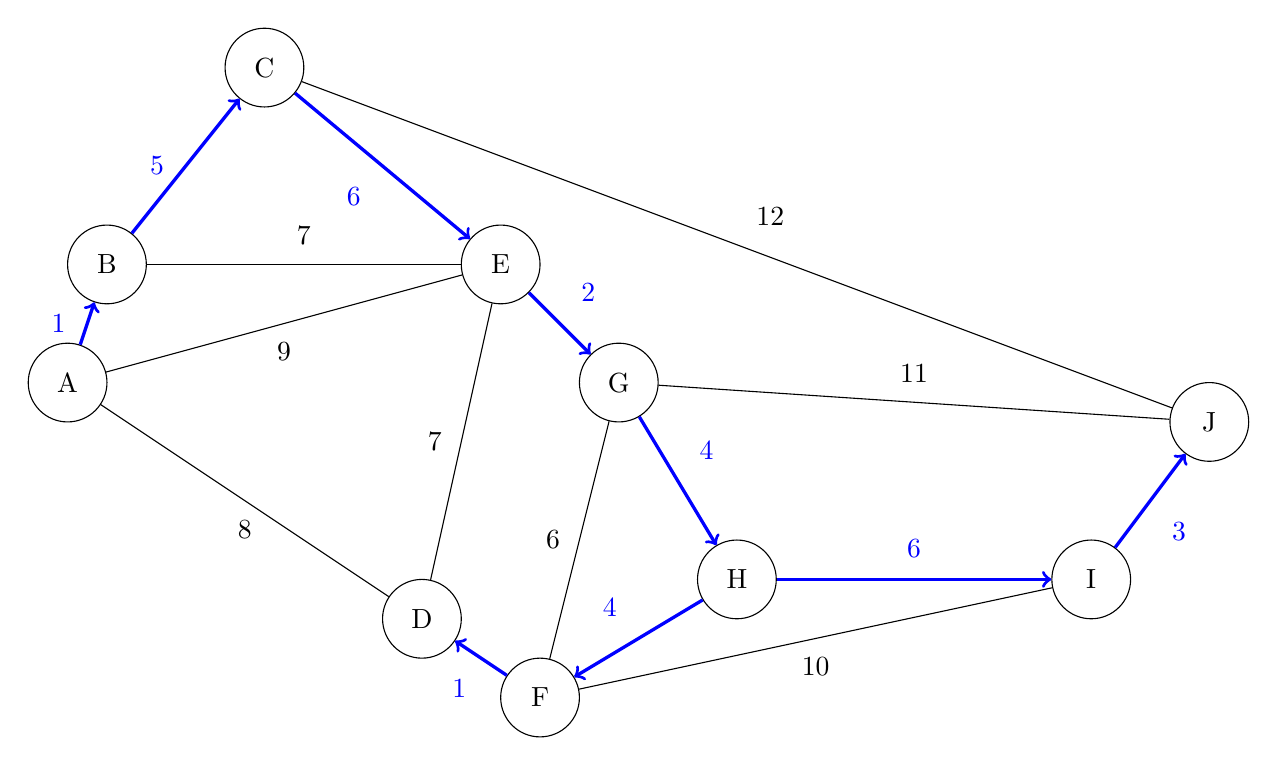
\begin{tikzpicture}[
                roundnode/.style={
                    draw, circle, minimum size=1cm
                }
            ]
            \node[roundnode] (A) at (0, 0) {A};
            \node[roundnode] (B) at (0.5, 1.5) {B};
            \node[roundnode] (C) at (2.5, 4) {C};
            \node[roundnode] (D) at (4.5, -3) {D};
            \node[roundnode] (E) at (5.5, 1.5) {E};
            \node[roundnode] (F) at (6, -4) {F};
            \node[roundnode] (G) at (7, 0) {G};
            \node[roundnode] (H) at (8.5, -2.5) {H};
            \node[roundnode] (I) at (13, -2.5) {I};
            \node[roundnode] (J) at (14.5, -0.5) {J};
            
            % nodes
            \draw[->, blue, very thick] (A) -- (B) node[midway, label={180:$1$}] {};
            \draw (A) -- (D) node[midway, label={270:$8$}] {};
            \draw (A) -- (E) node[midway, label={270:$9$}] {};
            \draw[->, blue, very thick] (B) -- (C) node[midway, label={180:$5$}] {};
            \draw (B) -- (E) node[midway, label={90:$7$}] {};
            \draw[->, blue, very thick] (C) -- (E) node[midway, label={225:$6$}] {};
            \draw (C) -- (J) node[midway, label={45:$12$}] {};
            \draw (D) -- (E) node[midway, label={180:$7$}] {};
            \draw[<-, blue, very thick] (D) -- (F) node[midway, label={250:$1$}] {};
            \draw[->, blue, very thick] (E) -- (G) node[midway, label={45:$2$}] {};
            \draw (F) -- (G) node[midway, label={180:$6$}] {};
            \draw[<-, blue, very thick] (F) -- (H) node[midway, label={135:$4$}] {};
            \draw (F) -- (I) node[midway, label={270:$10$}] {};
            \draw[->, blue, very thick] (G) -- (H) node[midway, label={45:$4$}] {};
            \draw (G) -- (J) node[midway, label={90:$11$}] {};
            \draw[->, blue, very thick] (H) -- (I) node[midway, label={90:$6$}] {};
            \draw[->, blue, very thick] (I) -- (J) node[midway, label={315:$3$}] {};
            \end{tikzpicture}
            }
            \caption{Prim's Minimum Spanning Tree, with cost of $32$}
            \label{fig:p4_2}
        \end{figure}

        \end{tcolorbox}
        
        \item Run \textbf{Kruskal’s} algorithm taught in 16 MST on the same graph to again find its MST. To answer this question, you need to follow the example in 16c\_Kruskal\_UF and provide the following information for each step:
        
        \begin{enumerate}[(1)]
            \item The current edge that is being tested, and the decision \textit{(i.e., ``YES" if this edge is added to the MST, ``NO" otherwise}).
            \item The current Union-Find data structure after adding the edge to MST if the decision is ``\textit{YES}"
            
            Also, upon completion of the algorithm, please:
            \item draw the final MST, and
            \item provide the minimum total route length (in kilometers) achieved by this MST.
        \end{enumerate}
        \begin{tcolorbox}[breakable]
        \begin{enumerate}[(1)]
            \item Step 1:
            edge: $\cbracket{A, B}$, decision: \textit{YES}
            \begin{figure}[H]
                \centering
                \begin{forest}
                tree, phantom
                [
                    [B, name=B
                        [A]
                    ]
                    [C, name=C]
                    [D, name=D]
                    [E, name=E]
                    [F, name=F]
                    [G, name=G]
                    [H, name=H]
                    [I, name=I]
                    [J, name=J]
                ]
                \foreach \i in {B, C, D, E, F, G, H, I, J}{
                    \draw[->] (\i) edge[loop above] (\i);
                }
                \end{forest}
            \end{figure}

            \item Step 2:
            edge: $\cbracket{D, F}$, decision: \textit{YES}
            \begin{figure}[H]
                \centering
                \begin{forest}
                tree, phantom
                [
                    [B, name=B
                        [A]
                    ]
                    [C, name=C]
                    [E, name=E]
                    [F, name=F
                        [D]
                    ]
                    [G, name=G]
                    [H, name=H]
                    [I, name=I]
                    [J, name=J]
                ]
                \foreach \i in {B, C, E, F, G, H, I, J}{
                    \draw[->] (\i) edge[loop above] (\i);
                }
                \end{forest}
            \end{figure}

            \item Step 3:
            edge: $\cbracket{E, G}$, decision: \textit{YES}
            \begin{figure}[H]
                \centering
                \begin{forest}
                tree, phantom
                [
                    [B, name=B
                        [A]
                    ]
                    [C, name=C]
                    [F, name=F
                        [D]
                    ]
                    [G, name=G
                        [E]
                    ]
                    [H, name=H]
                    [I, name=I]
                    [J, name=J]
                ]
                \foreach \i in {B, C, F, G, H, I, J}{
                    \draw[->] (\i) edge[loop above] (\i);
                }
                \end{forest}
            \end{figure}

            \item Step 4:
            edge: $\cbracket{I, J}$, decision: \textit{YES}
            \begin{figure}[H]
                \centering
                \begin{forest}
                tree, phantom
                [
                    [B, name=B
                        [A]
                    ]
                    [C, name=C]
                    [F, name=F
                        [D]
                    ]
                    [G, name=G
                        [E]
                    ]
                    [H, name=H]
                    [J, name=J
                        [J]
                    ]
                ]
                \foreach \i in {B, C, F, G, H, J}{
                    \draw[->] (\i) edge[loop above] (\i);
                }
                \end{forest}
            \end{figure}

            \item Step 5:
            edge: $\cbracket{F, H}$, decision: \textit{YES}
            \begin{figure}[H]
                \centering
                \begin{forest}
                tree, phantom
                [
                    [B, name=B
                        [A]
                    ]
                    [C, name=C]
                    [F, name=F
                        [D]
                        [H]
                    ]
                    [G, name=G
                        [E]
                    ]
                    [J, name=J
                        [I]
                    ]
                ]
                \foreach \i in {B, C, F, G, J}{
                    \draw[->] (\i) edge[loop above] (\i);
                }
                \end{forest}
            \end{figure}

            \item Step 6:
            edge: $\cbracket{G, H}$, decision: \textit{YES}
            \begin{figure}[H]
                \centering
                \begin{forest}
                tree, phantom
                [
                    [B, name=B
                        [A]
                    ]
                    [C, name=C]
                    [F, name=F
                        [D]
                        [H]
                        [G
                            [E]
                        ]
                    ]
                    [J, name=J
                        [I]
                    ]
                ]
                \foreach \i in {B, C, F, J}{
                    \draw[->] (\i) edge[loop above] (\i);
                }
                \end{forest}
            \end{figure}

            \item Step 7:
            edge: $\cbracket{B, C}$, decision: \textit{YES}
            \begin{figure}[H]
                \centering
                \begin{forest}
                tree, phantom
                [
                    [B, name=B
                        [A]
                        [C]
                    ]
                    [F, name=F
                        [D]
                        [H]
                        [G
                            [E]
                        ]
                    ]
                    [J, name=J
                        [I]
                    ]
                ]
                \foreach \i in {B, F, J}{
                    \draw[->] (\i) edge[loop above] (\i);
                }
                \end{forest}
            \end{figure}

            \item Step 8:
            edge: $\cbracket{C, E}$, decision: \textit{YES}
            \begin{figure}[H]
                \centering
                \begin{forest}
                tree, phantom
                [
                    [F, name=F
                        [B
                            [A]
                            [C]
                        ]
                        [D]
                        [H]
                        [G
                            [E]
                        ]
                    ]
                    [J, name=J
                        [I]
                    ]
                ]
                \foreach \i in {F, J}{
                    \draw[->] (\i) edge[loop above] (\i);
                }
                \end{forest}
            \end{figure}

            \item Step 9:
            edge: $\cbracket{F, G}$, decision: \textit{NO}

            \item Step 10:
            edge: $\cbracket{H, I}$, decision: \textit{YES}
            \begin{figure}[H]
                \centering
                \begin{forest}
                tree, phantom
                [
                    [F, name=F
                        [B
                            [A]
                            [C]
                        ]
                        [D]
                        [H]
                        [G
                            [E]
                        ]
                        [J
                            [I]
                        ]
                    ]
                ]
                \foreach \i in {F}{
                    \draw[->] (\i) edge[loop above] (\i);
                }
                \end{forest}
            \end{figure}

            \item Step 11:
            edge: $\cbracket{B, E}$, decision: \textit{NO}

            \item Step 12:
            edge: $\cbracket{D, E}$, decision: \textit{NO}

            \item Step 13:
            edge: $\cbracket{A, D}$, decision: \textit{NO}

            \item Step 14:
            edge: $\cbracket{A, E}$, decision: \textit{NO}

            \item Step 15:
            edge: $\cbracket{F, I}$, decision: \textit{NO}

            \item Step 16:
            edge: $\cbracket{G, J}$, decision: \textit{NO}

            \item Step 17:
            edge: $\cbracket{C, J}$, decision: \textit{NO}
        \end{enumerate}
        \begin{figure}[H]
            \centering
            \resizebox{0.7\linewidth}{!}{
            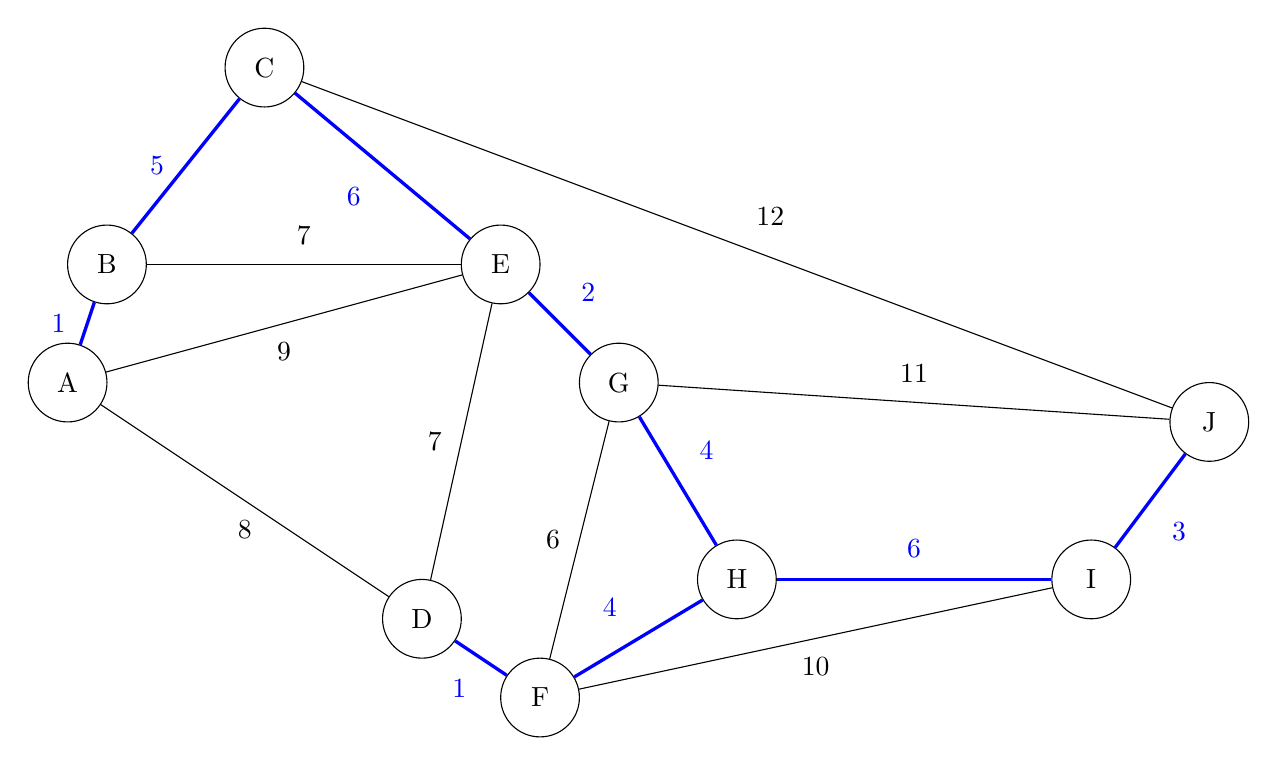
\begin{tikzpicture}[
                roundnode/.style={
                    draw, circle, minimum size=1cm
                }
            ]
            \node[roundnode] (A) at (0, 0) {A};
            \node[roundnode] (B) at (0.5, 1.5) {B};
            \node[roundnode] (C) at (2.5, 4) {C};
            \node[roundnode] (D) at (4.5, -3) {D};
            \node[roundnode] (E) at (5.5, 1.5) {E};
            \node[roundnode] (F) at (6, -4) {F};
            \node[roundnode] (G) at (7, 0) {G};
            \node[roundnode] (H) at (8.5, -2.5) {H};
            \node[roundnode] (I) at (13, -2.5) {I};
            \node[roundnode] (J) at (14.5, -0.5) {J};
            
            % nodes
            \draw[blue, very thick] (A) -- (B) node[midway, label={180:$1$}] {};
            \draw (A) -- (D) node[midway, label={270:$8$}] {};
            \draw (A) -- (E) node[midway, label={270:$9$}] {};
            \draw[blue, very thick] (B) -- (C) node[midway, label={180:$5$}] {};
            \draw (B) -- (E) node[midway, label={90:$7$}] {};
            \draw[blue, very thick] (C) -- (E) node[midway, label={225:$6$}] {};
            \draw (C) -- (J) node[midway, label={45:$12$}] {};
            \draw (D) -- (E) node[midway, label={180:$7$}] {};
            \draw[blue, very thick] (D) -- (F) node[midway, label={250:$1$}] {};
            \draw[blue, very thick] (E) -- (G) node[midway, label={45:$2$}] {};
            \draw (F) -- (G) node[midway, label={180:$6$}] {};
            \draw[blue, very thick] (F) -- (H) node[midway, label={135:$4$}] {};
            \draw (F) -- (I) node[midway, label={270:$10$}] {};
            \draw[blue, very thick] (G) -- (H) node[midway, label={45:$4$}] {};
            \draw (G) -- (J) node[midway, label={90:$11$}] {};
            \draw[blue, very thick] (H) -- (I) node[midway, label={90:$6$}] {};
            \draw[blue, very thick] (I) -- (J) node[midway, label={315:$3$}] {};
            \end{tikzpicture}
            }
            \caption{Kruskal's Minimum Spanning Tree, with cost of $32$}
            \label{fig:p4_3}
        \end{figure}

        \end{tcolorbox}
    \end{enumerate}
    
    \item Run \textbf{Dijkstra’s} Algorithm on the same graph to find the shortest path from Santa Lucia Train Station (node $B$) to all the other tourist destinations.
    
    To answer this question, you need to follow the example in 17c\_Dijkstra\_Worked\_Example and provide the following information for each step:
    \begin{enumerate}[(1)]
        \item A table that tracks the distance value $(d[u])$ and parent $(p[u])$ of each node.
        Also, upon completion of the algorithm, please:
        \item draw the final shortest-path tree.
    \end{enumerate}
    \begin{tcolorbox}[breakable]
    \begin{enumerate}[(1)]
                \item Step 1:
                \begin{table}[H]
                    \centering
                    \begin{tabular}{c|cccccccccc}
                        \hline
                        $u$ & A & B & C & D & E & F & G & H & I & J \\
                        $d[u]$ & 1 & 0 & $\infty$ & $\infty$ & $\infty$ & $\infty$ & $\infty$ & $\infty$ & $\infty$ & $\infty$ \\
                        $p[u]$ & B & - & - & - & - & - & - & - & - & - \\
                        \hline
                    \end{tabular}
                \end{table}
                

                \item Step 2:
                \begin{table}[H]
                    \centering
                    \begin{tabular}{c|cccccccccc}
                        \hline
                        $u$ & A & B & C & D & E & F & G & H & I & J \\
                        $d[u]$ & 1 & 0 & 5 & $\infty$ & $\infty$ & $\infty$ & $\infty$ & $\infty$ & $\infty$ & $\infty$ \\
                        $p[u]$ & B & - & B & - & - & - & - & - & - & - \\
                        \hline
                    \end{tabular}
                \end{table}
                

                \item Step 3:
                \begin{table}[H]
                    \centering
                    \begin{tabular}{c|cccccccccc}
                        \hline
                        $u$ & A & B & C & D & E & F & G & H & I & J \\
                        $d[u]$ & 1 & 0 & 5 & $\infty$ & 7 & $\infty$ & $\infty$ & $\infty$ & $\infty$ & $\infty$ \\
                        $p[u]$ & B & - & B & - & B & - & - & - & - & - \\
                        \hline
                    \end{tabular}
                \end{table}
                

                \item Step 4:
                \begin{table}[H]
                    \centering
                    \begin{tabular}{c|cccccccccc}
                        \hline
                        $u$ & A & B & C & D & E & F & G & H & I & J \\
                        $d[u]$ & 1 & 0 & 5 & 9 & 7 & $\infty$ & $\infty$ & $\infty$ & $\infty$ & $\infty$ \\
                        $p[u]$ & B & - & B & A & B & - & - & - & - & - \\
                        \hline
                    \end{tabular}
                \end{table}
                

                \item Step 5:
                \begin{table}[H]
                    \centering
                    \begin{tabular}{c|cccccccccc}
                        \hline
                        $u$ & A & B & C & D & E & F & G & H & I & J \\
                        $d[u]$ & 1 & 0 & 5 & 9 & 7 & $\infty$ & $\infty$ & $\infty$ & $\infty$ & 17 \\
                        $p[u]$ & B & - & B & A & B & - & - & - & - & C \\
                        \hline
                    \end{tabular}
                \end{table}
                

                \item Step 6:
                \begin{table}[H]
                    \centering
                    \begin{tabular}{c|cccccccccc}
                        \hline
                        $u$ & A & B & C & D & E & F & G & H & I & J \\
                        $d[u]$ & 1 & 0 & 5 & 9 & 7 & $\infty$ & 9 & $\infty$ & $\infty$ & 17 \\
                        $p[u]$ & B & - & B & A & B & - & E & - & - & C \\
                        \hline
                    \end{tabular}
                \end{table}
                

                \item Step 7:
                \begin{table}[H]
                    \centering
                    \begin{tabular}{c|cccccccccc}
                        \hline
                        $u$ & A & B & C & D & E & F & G & H & I & J \\
                        $d[u]$ & 1 & 0 & 5 & 9 & 7 & 15 & 9 & $\infty$ & $\infty$ & 17 \\
                        $p[u]$ & B & - & B & A & B & G & E & - & - & C \\
                        \hline
                    \end{tabular}
                \end{table}
                

                \item Step 8:
                \begin{table}[H]
                    \centering
                    \begin{tabular}{c|cccccccccc}
                        \hline
                        $u$ & A & B & C & D & E & F & G & H & I & J \\
                        $d[u]$ & 1 & 0 & 5 & 9 & 7 & 15 & 9 & 13 & $\infty$ & 17 \\
                        $p[u]$ & B & - & B & A & B & G & E & G & - & C \\
                        \hline
                    \end{tabular}
                \end{table}
                

                \item Step 9:
                \begin{table}[H]
                    \centering
                    \begin{tabular}{c|cccccccccc}
                        \hline
                        $u$ & A & B & C & D & E & F & G & H & I & J \\
                        $d[u]$ & 1 & 0 & 5 & 9 & 7 & 10 & 9 & 13 & $\infty$ & 17 \\
                        $p[u]$ & B & - & B & A & B & D & E & G & - & C \\
                        \hline
                    \end{tabular}
                \end{table}
                

                \item Step 10:
                \begin{table}[H]
                    \centering
                    \begin{tabular}{c|cccccccccc}
                        \hline
                        $u$ & A & B & C & D & E & F & G & H & I & J \\
                        $d[u]$ & 1 & 0 & 5 & 9 & 7 & 10 & 9 & 13 & 20 & 17 \\
                        $p[u]$ & B & - & B & A & B & D & E & G & F & C \\
                        \hline
                    \end{tabular}
                \end{table}
                

                \item Step 11:
                \begin{table}[H]
                    \centering
                    \begin{tabular}{c|cccccccccc}
                        \hline
                        $u$ & A & B & C & D & E & F & G & H & I & J \\
                        $d[u]$ & 1 & 0 & 5 & 9 & 7 & 10 & 9 & 13 & 19 & 17 \\
                        $p[u]$ & B & - & B & A & B & D & E & G & H & C \\
                        \hline
                    \end{tabular}
                \end{table}
    \end{enumerate}
    \begin{figure}[H]
        \centering
        \resizebox{0.7\linewidth}{!}{
        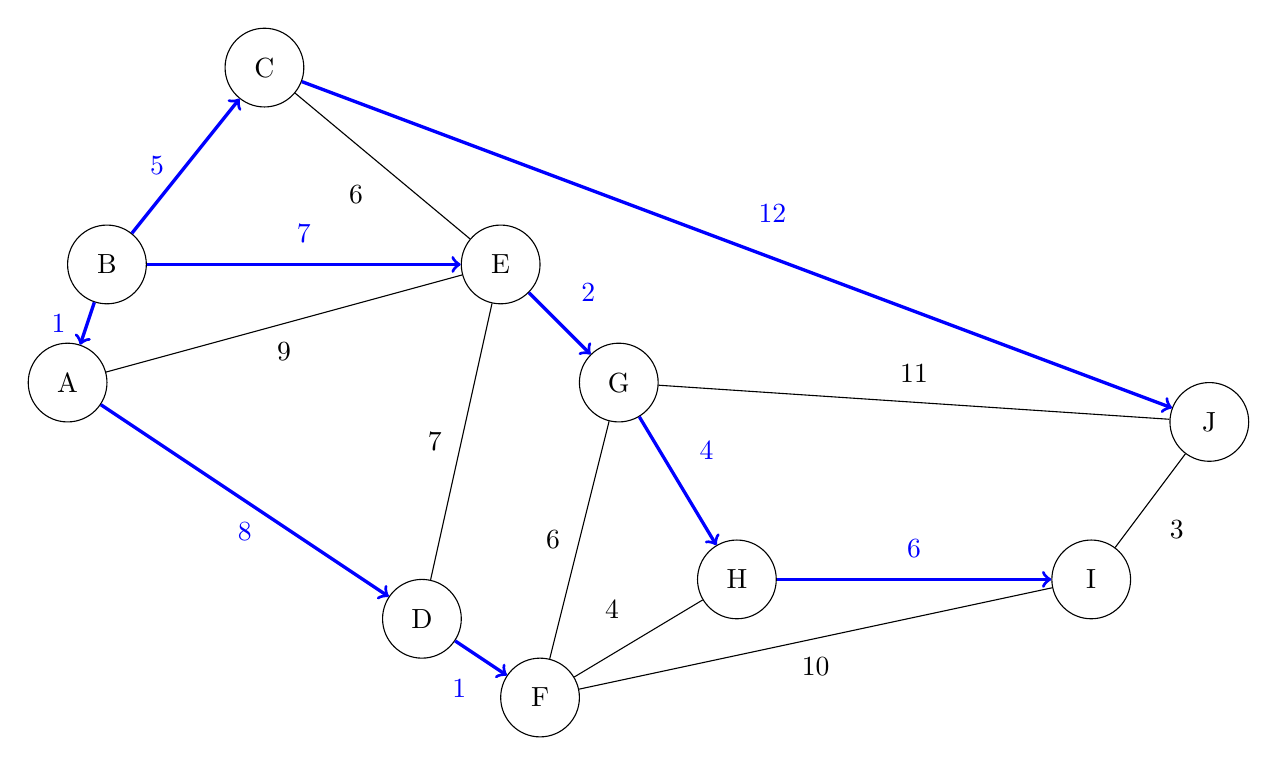
\begin{tikzpicture}[
            roundnode/.style={
                draw, circle, minimum size=1cm
            }
        ]
        \node[roundnode] (A) at (0, 0) {A};
        \node[roundnode] (B) at (0.5, 1.5) {B};
        \node[roundnode] (C) at (2.5, 4) {C};
        \node[roundnode] (D) at (4.5, -3) {D};
        \node[roundnode] (E) at (5.5, 1.5) {E};
        \node[roundnode] (F) at (6, -4) {F};
        \node[roundnode] (G) at (7, 0) {G};
        \node[roundnode] (H) at (8.5, -2.5) {H};
        \node[roundnode] (I) at (13, -2.5) {I};
        \node[roundnode] (J) at (14.5, -0.5) {J};
        
        % nodes
        \draw[<-, blue, very thick] (A) -- (B) node[midway, label={180:$1$}] {};
        \draw[->, blue, very thick] (A) -- (D) node[midway, label={270:$8$}] {};
        \draw (A) -- (E) node[midway, label={270:$9$}] {};
        \draw[->, blue, very thick] (B) -- (C) node[midway, label={180:$5$}] {};
        \draw[->, blue, very thick] (B) -- (E) node[midway, label={90:$7$}] {};
        \draw (C) -- (E) node[midway, label={225:$6$}] {};
        \draw[->, blue, very thick] (C) -- (J) node[midway, label={45:$12$}] {};
        \draw (D) -- (E) node[midway, label={180:$7$}] {};
        \draw[->, blue, very thick] (D) -- (F) node[midway, label={250:$1$}] {};
        \draw[->, blue, very thick] (E) -- (G) node[midway, label={45:$2$}] {};
        \draw (F) -- (G) node[midway, label={180:$6$}] {};
        \draw (F) -- (H) node[midway, label={135:$4$}] {};
        \draw (F) -- (I) node[midway, label={270:$10$}] {};
        \draw[->, blue, very thick] (G) -- (H) node[midway, label={45:$4$}] {};
        \draw (G) -- (J) node[midway, label={90:$11$}] {};
        \draw[->, blue, very thick] (H) -- (I) node[midway, label={90:$6$}] {};
        \draw (I) -- (J) node[midway, label={315:$3$}] {};
        \end{tikzpicture}
        }
        \caption{Djikstra's Shortest Path Tree}
        \label{fig:p4_1}
    \end{figure}

    \end{tcolorbox}
\end{enumerate}
\end{section}
\end{document}
